\chapter*{Contribuții} 
\addcontentsline{toc}{chapter}{Contribuții}

Analizând produsele deja existente bazate pe o idee similară am constatat că fiecare dintre ele prezintă un neajuns.
Multe aplicații sunt concepute, spre exemplu, doar pentru sistemul de operare Windows.
O analiză a cotei de piață pentru sistemele de operare pentru sisteme desktop ne indică faptul că există un număr semnificativ de utilizatori care nu folosesc mașini ce rulează Windows.
Așadar, aplicația propusă este \emph{cross-platform}, putând fi rulată pe cele mai importante 3 sisteme de operare: Windows, MacOS și Linux.

\begin{figure}[h]
    \centering
    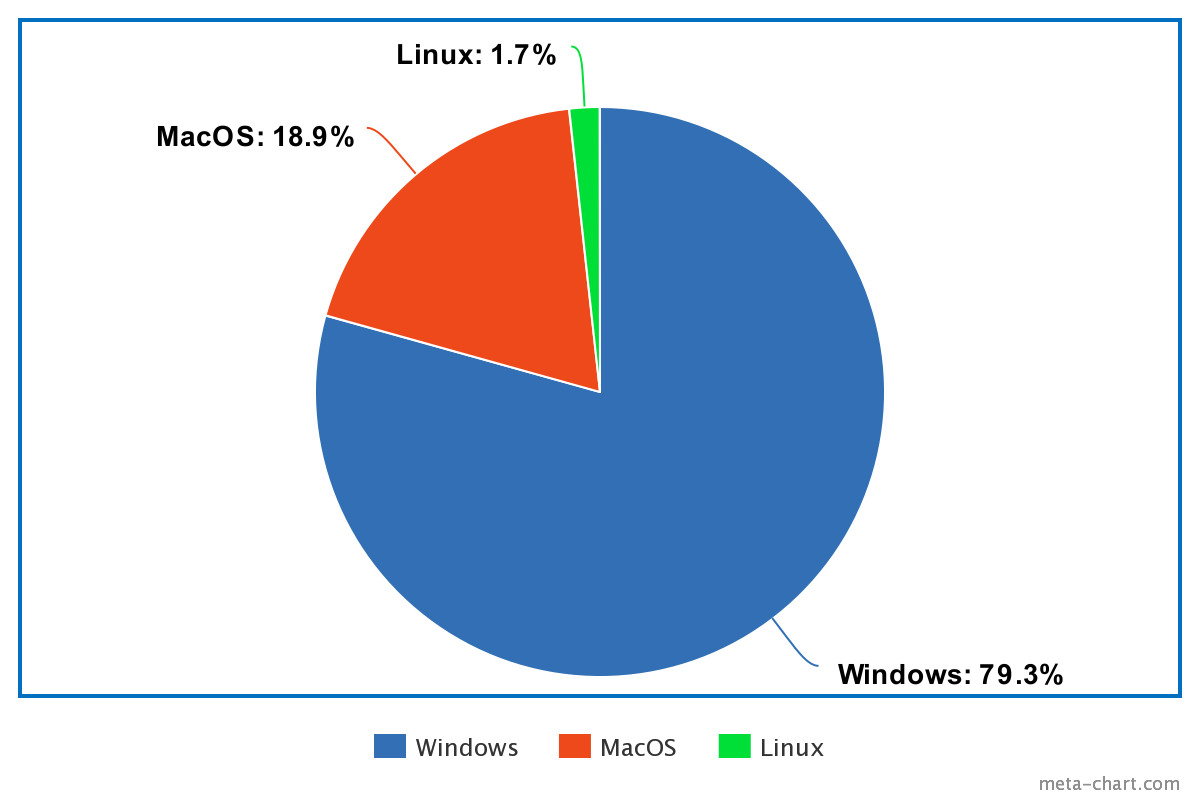
\includegraphics[width=\textwidth]{os.png}
    \caption{Distribuție a sistemelor de operare desktop în Mai, 2020. Mulți utilizatori nu folosesc Windows. Date preluate de pe \href{https://gs.statcounter.com/os-market-share/desktop/worldwide}{StatCounter GlobalStats}}
\end{figure}

Un alt punct important este că unele aplicații necesită camere speciale sau senzori speciali, ceea ce aduce un cost în plus și poate fi un impediment în utilizarea aplicației.
Lucrarea de față nu necesită decât o cameră webcam, hardware care este deja existent pe orice laptop comercializat astăzi sau care poate fi atașat unui calculator obișnuit pentru un cost redus.

O ultimă mențiune este legată de diferențele fizionomice dintre persoane.
În acest sens, aplicația se poate ``adapta'' fizionomiei fiecărui utilizator, întrucât pentru a analiza punctul de privire al utilizatorului sunt folosite imagini cu acesta.
Acest lucru aduce un pas în plus pentru ``configurarea'' aplicației (colectarea de date), dar va rezulta într-o experiență mai robustă pentru fiecare utilizator în parte.